\chapter{Drawing the Planets and Orbits}
\section{Planets}
Drawing the planets is generally very simple: at first we create a sphere using the {\em sphere} function which gives us the coordinates {\em x}, {\em y} and {\em z} of each corner of the sphere while taking the  resolution as the argument. The resolution defines how smooth the surface of the sphere is. For example: a resolution of 50 generates a spheres composed of 50 equally wide rings with 50 equally big surfaces. Following images shows how the spheres react to different resolutions:

\begin{center}
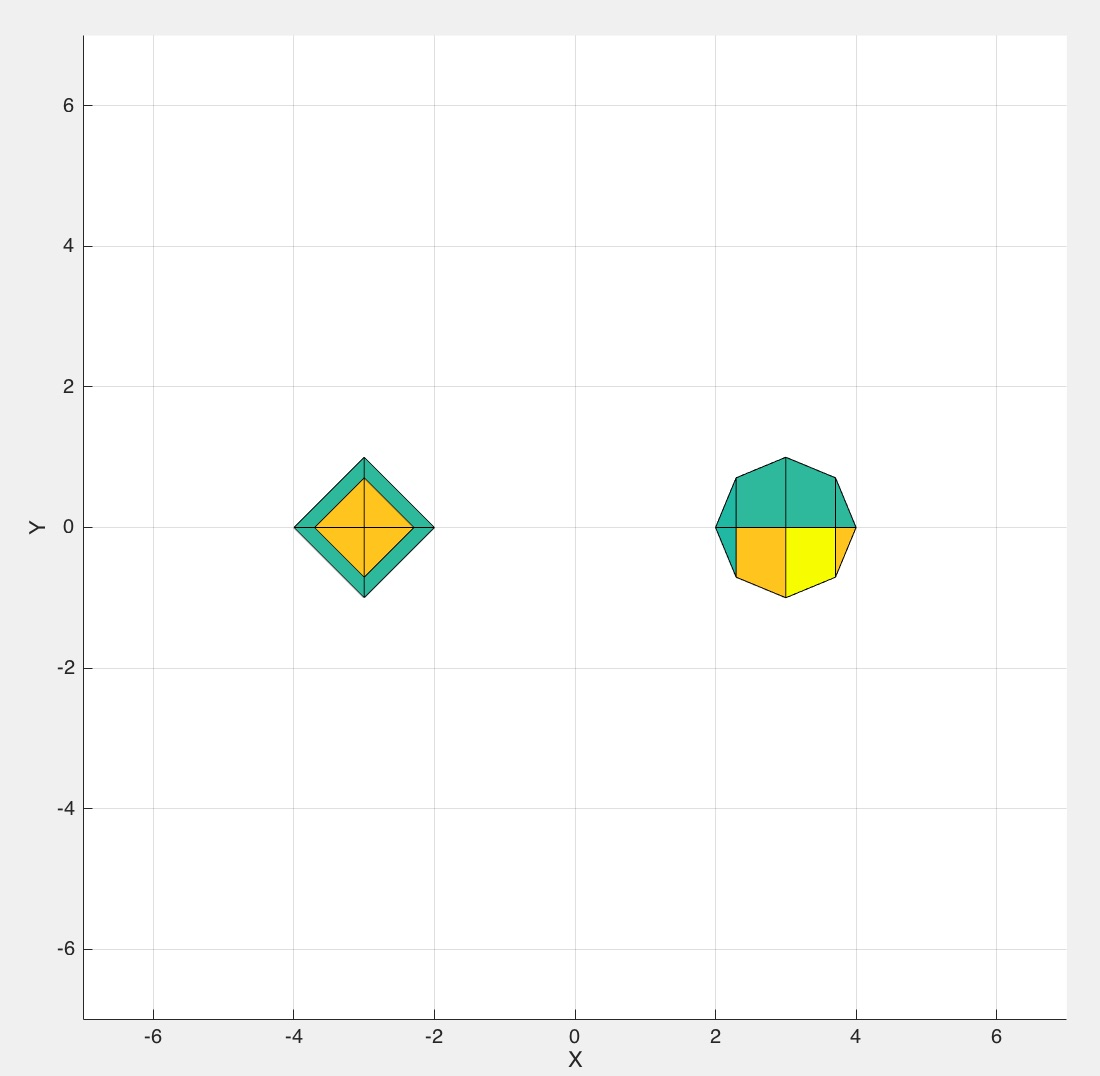
\includegraphics[width=0.45\textwidth]{imgs/drawing_planets_orbits/spheres_res4.jpg}
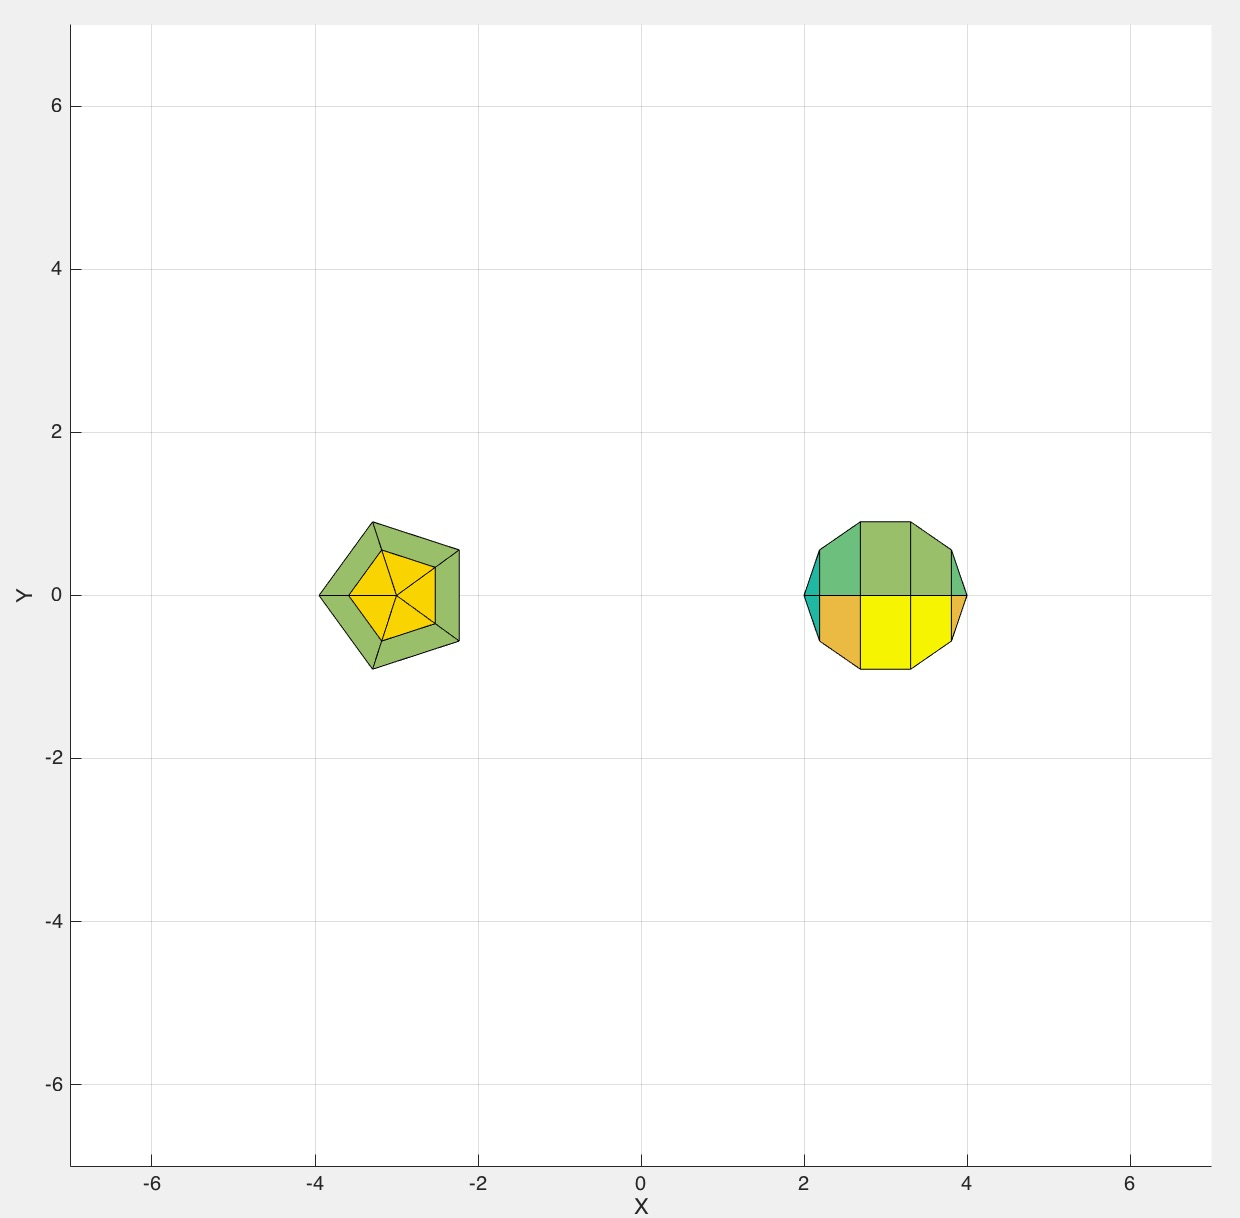
\includegraphics[width=0.45\textwidth]{imgs/drawing_planets_orbits/spheres_res5.jpg}\\
\textit{Left: a sphere with resolution 4 (top and side view); Right: a sphere with resolution 5 (top and side view)}
\end{center}

We then manipulate the position values to scale and move the sphere as needed. We do this by multiplying the position matrices with a factor and then adding a constant to move it to the correct position.\\

Next we load the textures from an image using various \matlab{} functions: first we read the image of a map of the planet using {\em imread}. Then we convert the data to doubles using {\em im2double}. Next we use {\em imresize} to adjust the image the size of the planet. We then only have to flip the data upside down to correctly display the texture. This is done using the {\em flipud} function. Further details for these function can be found in the help pages of each function.\\

Last but no least we create a surface object, or the 'planet', using the {\em surf} function by passing the position matrices and the textures. We can then use this object to move and rotated the planet.

Following {\em MatLab} code draws a simple sphere with a texture as described above:
\begin{framed}\begin{verbatim}
[x,y,z] = sphere(resolution);
x = x*scale(1) + pos(1); y = y*scale(2) + pos(2); z = z*scale(3) + pos(3);

texture = flipud(imresize(im2double(imread(imgFile)),size(x)));
planet = surf(x, y, z, texture,'EdgeColor', 'none');
\end{verbatim}\end{framed}
{\em pos} and {\em scale} are vectors containing the coordinates of the center of the planet and factors for stretching the planet in {\em x}, {\em y} and {\em z} directions. {\em imgFile} is a string containing the path to the textures of the planet and {\em resolution} is an integer for the resolution of the sphere as described above.

\subsection{Rings}
Some planets, in our case only saturn, have rings of water ice and rocky material circling them. To respect the thickness of such rings and for simplicity we created them using a torus and squished it to make it thiner. A torus is described as follows:

\begin{align*}
x(\theta, \varphi) = (R + r*\cos(\theta) * \cos(\varphi)\\
y(\theta, \varphi) = (R + r*\cos(\theta) * \sin(\varphi)\\
x(\theta, \varphi) = r*\sin(\varphi)
\end{align*}

$\theta$, $\varphi$ are angles which make a full circle, so that their values start and end at the same point,\\
R is the distance from the center of the tube to the center of the torus,\\
r is the radius of the tube.

In \matlab{} this looks some what like this:
\begin{framed}\begin{verbatim}
phi = linspace(0,2*pi,resolution)';
alpha = linspace(0,2*pi,resolution*10)';

tmp = [R + r*cos(phi), r*sin(phi)];
x = cos(alpha)*tmp(:,1)';
y = sin(alpha)*tmp(:,1)';
z = tmp(:,2)';
z = z(ones(1,length(alpha)),:);
\end{verbatim}\end{framed}
The rest for drawing the ring is the same as for drawing the planets: we move and scale the ring using vectors containing the position of the center and factors for each direction and then create a surface object with the textures of the ring. Only the textures are slightly different compared to the planets. While the planets use a map, the ring has to be only a portion of the ring mirrored along the inner {\em 'edge'} of the ring.


\section{Orbits}
We decided to use circular orbits for our modle, instead of simulating them and calculating the trajectory. Thus drawing the trajectory of each planet was made a lot easier.  The function {\em getPlanetOrbit} draws a simple circle in a 3 dimensional room. The function has the following attributes:
\begin{itemize}
  \item Center: stands for the middle of the circle
  \item Normal: stands for direction that the circle is tilted
  \item Radius: radius of the circle
  \item Color: color of the circle \ldots
\end{itemize}


\begin{framed}\begin{verbatim}
theta = 0:0.01:(2*pi+0.01);
v = null(normal);
points = repmat(center',1,size(theta,2))+radius*(v(:,1)*cos(theta)+v(:,2)*sin(theta));
orbit = plot3(points(1,:),points(2,:),points(3,:),'Color',color);
\end{verbatim}\end{framed}

% ================================
\pagebreak
\section{Key Values for the Modle}
As said before, we tryed to use realistic values and scales for the modle. Listed in the following two chapters are the values we ended up using. We gathered the data from: \hyperref[space-facts.com]{http://space-facts.com/}

\subsection{Distances}
\begin{center}
    \begin{tabular}{| l | l | l | l |}
    \hline
    Planet & Distance [km] & Distance [AU] & Scale Factor \\ \hline
    Mercury & 57'909'227 & 0.39 & 0.39 \\ \hline
    Venus & 108'209'475 & 0.73 & 0.73 \\ \hline
    Earth & 149'598'262 & 1 & 1 \\ \hline
    Moon & 384'400 & 0.0025 & 0.0025 \\ \hline
    Mars & 227'943'824 & 1.38 & 1.38 \\ \hline
    Jupiter & 778'340'821 & 5.20 & 5.20 \\ \hline
    Saturn & 1'426'666'422 & 9.58 & 9.58 \\ \hline
    Uranus & 2'870'658'186 & 19.22 & 19.22 \\ \hline
    Neptune & 4'498'396'441 & 30.10 & 30.10 \\
    \hline
    \end{tabular}\\
    \textit{The distances are all the average distance from the sun.\\
    Except for the moon, whose distance is the average distance from earth.}
\end{center}


\subsection{Sizes}
\begin{center}
    \begin{tabular}{| l | l | l |}
    \hline
    Planet & Diameter [km] & Scale Factor \\ \hline
    Sun & 1'392'684 & 109.18 \\ \hline
    Mercury & 4'879 & 0.38 \\ \hline
    Venus & 12'104 & 0.95 \\ \hline
    Earth & 12'756 & 1 \\ \hline
    Moon & 3'475 & 0.27 \\ \hline
    Mars & 6'805 & 0.53 \\ \hline
    Jupiter & 142'984 & 11.21 \\ \hline
    Saturn & 120'536 & 9.45 \\ \hline
    Uranus & 51'118 & 4.01 \\ \hline
    Neptune & 49'528 & 3.88 \\
    \hline
    \end{tabular}\\
    \textit{The diameters used are the equatorial diameters of the planets.\\
    The scale factor used is log10 of the value in this table.}
\end{center}


\subsection{Speed}
\begin{center}
    \begin{tabular}{| l | l | l |}
    \hline
    Planet & Earth days / year & Scale Factor \\ \hline
    Mercury & 87.97 & 4.1521 \\ \hline
    Venus & 224.7 & 1.6255 \\ \hline
    Earth & 365.26 & 1 \\ \hline
    Moon & 27.3 & 13.3795 \\ \hline
    Mars & 686.98 & 0.5317 \\ \hline
    Jupiter & 4332.82 & 0.0843 \\ \hline
    Saturn & 10755.7 & 0.034 \\ \hline
    Uranus & 30687.15 & 0.0119 \\ \hline
    Neptune & 60190.03 & 0.0061 \\
    \hline
    \end{tabular}\\
    \textit{The scale factor is used for the orbit speed.\\
    Therefor less days mean faster orbit speed.}
\end{center}
